%!TEX root = ../dokumentation.tex

\chapter{Example LAN Application Implementation}\label{cha:ExampleLAN}

To develop an application, a plan is required that guides the development process, which is usually at least an architecture concept.
The architecture is created based on the application components (cf. chapter \ref{cha:Requirement:lanpartyapplication}) and the technologies selected (cf. chapter \ref{cha:Implementation}).
To fully exploit the potential of the technologies, the resulting \ac{LAN} Application will be implemented using the microservice architecture.
An important principle is the single responsibility principle form Robert C. Martin’s: \cite[p.~4]{Bruce.2019}

\begin{quote}
	Gather together the things that change for the same reasons. Separate those things that
	change for different reasons.
\end{quote}

Taking this principle into account and combining it with the application components, each component will be isolated into its own microservice.
Other microservice attributes that should be considered are, for example, that a microservice should know little about other microservice, they should be independently deployable and replaceable.
These attributes leads to providing one database per microservice \cite[p.~4ff.]{Bruce.2019}.

Another important part to consider when building a microservice architecture it the fact that it is a distributed system.
False assumptions like the network is reliable must be avoided \cite[p.~16]{Bruce.2019}.
Therefore, \ac{QoS} \textit{at-least-once} will be used and considered when creating the architecture.
It was chosen because the application must be consistent and availability can be achieved by scaling.

These are the general guidelines for creating the architecture, next is to evaluate the use of the different communication technologies.
The selected technologies are \ac{REST} for synchronous messaging and RabbitMQ for asynchronous messaging.
Synchronous messaging is used for communication where direct feedback is required, such as client-server communication.
Asynchronous messaging, on the other hand, is used to decouple communication partners.
This allows dynamic growth and parallel work distribution within the microservice application \cite[p.~62f.]{Bruce.2019}.
Therefore, asynchronous messaging is used for inter-service communication.

Another common principle in microservice architectures is the use of a boundary layer that provides abstraction over internal complexity and change \cite[p.~66]{Bruce.2019}.
Therefore, an \ac{API} Gateway will be used as single entry point for the application.
This has advantages such as centralized handling of authentication, routing and transmission transformations.
It also minimizes the exposed surface area of the application \cite[p.~68f.]{Bruce.2019}.

Now that the general structure of the services has been described, one last part must be described, namely the \ac{UI}.
The user interface can be either a web page or full fledged application, and both can be implemented via a monolith or micro frontend approach.
The \ac{UI} will have cross microservice concerns to ensure usability \cite[p.~71f.]{Bruce.2019}.
So, since this work focuses on communication technologies for a microservice environment, the approach used for the \ac{UI} should hardly affect communication.
Therefore, a monolithic web page will be realized because it is simple to realize, and the authors have experience with this kind of application.

The architecture of the \ac{LAN} application can be divided into two parts.
The first part shows the synchronous communication and the second part shows the asynchronous communication.

\textbf{Overview of the Synchronous Messaging Architecture}

An architectural overview of the synchronous messaging is shown in Figure \ref{img:lansyncoverview}.
An \ac{API} gateway, which will be \textit{Nginx}, abstracts the microservice system.
Depending on the domain used, \textit{Nginx} forwards the requests to the microservice system or to \textit{Grafana}.
This means that \textit{domain.de} will return the \ac{LAN} application and \textit{metric.domain.de} will return \textit{Grafana}.
Each microservice has its own REST endpoint which is accessible via \textit{/api/<name of service>}.
\textit{Nginx} will use the service name within the \ac{URL} to route the request and truncate the \ac{URL}.
For example, a request \textit{domain.de/api/account/1} will be routed to the account microservice and the forwarded request will be \textit{<ip of account>/1}.

For logging purposes, Prometheus will be used.
Each microservice will collect metrics about requests and provide an endpoint for Prometheus.
This is visualized by the red box attached to each microservice.
Finally, each microservice has its one MongoDB database.
For simplicity, all databases run in one instance, but they could be distributed across different MongoDB instances.

\begin{figure}
	\centering
	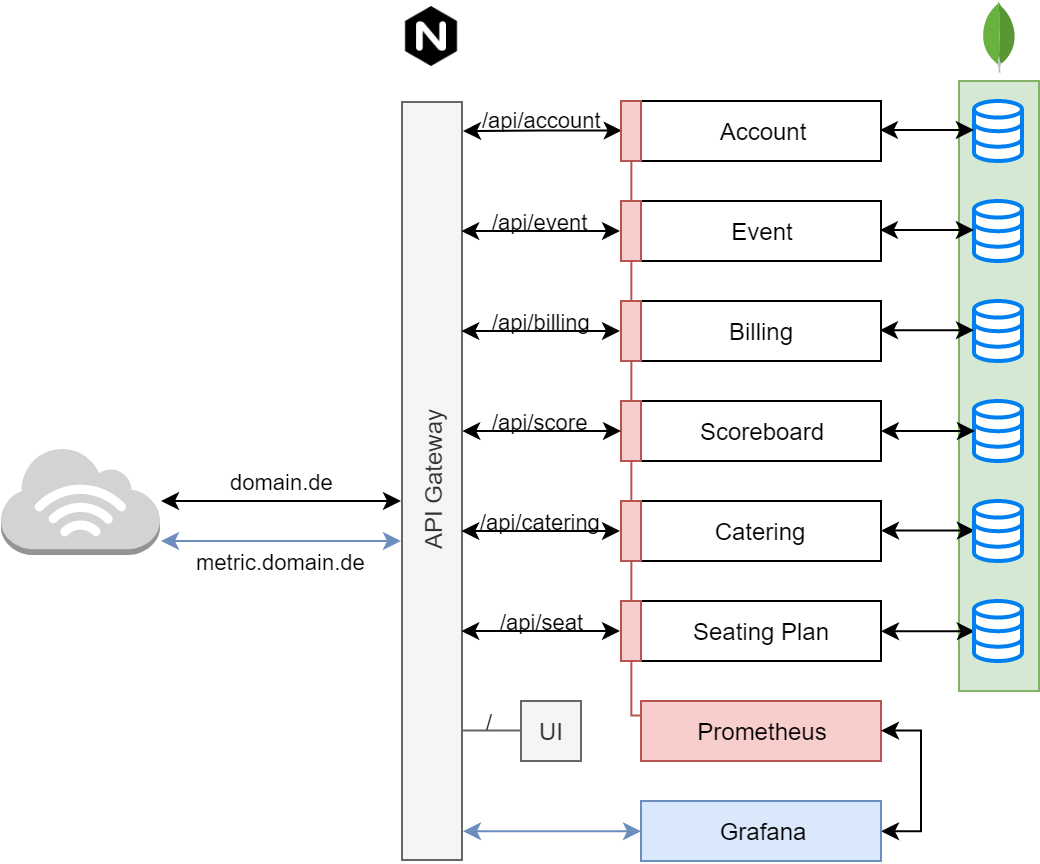
\includegraphics[width=0.7\textwidth, height=0.9\textheight, keepaspectratio]{LAN_Application_REST.png}
	\caption{LAN application synchronous messaging architecture overview}
	\label{img:lansyncoverview}
\end{figure}

\textbf{Asynchronous Messaging Events}

Before describing asynchronous messaging, it is important to note that every microservice must be able to validate any request from the client by itself.
Therefore, the microservice needs the necessary information for any validation itself and must not be dependent on other microservice.
This leads to the distribution of shared information and that is the main concern of the following overview of asynchronous messaging.

Figure \ref{img:lanasyncevents} is a simplified overview of the available topics and how the microservices interact with them.
An important design decision was made to allow the flexibility described above.
Every microservice must subscribe to the \textit{Account} and \textit{Event} topics, to receive all \textit{created} events (not included in the image for readability).
This distributes the event and account ID's to all microservice.
These ID's are the center of almost all operation.

In Figure \ref{img:lanasyncevents}, most of the publish arrows numbered.
Each number is associated with a reason for this connection, which is described in the following list.
\begin{enumerate}
	\item \textit{Events} and \textit{catering} can cost money and must therefore inform \textit{billing}
	\item The \textit{event} must know when the fees for an event are payed
	\item The \textit{catering} and \textit{searing plan} must know when an account has registered for an event. This will enable there functionality.
	\item The \textit{scoreboard} must know when an event starts and when it ends
	\item \textit{Scoreboard} publishes a summery of the event results to event and account topics
\end{enumerate}

\begin{figure}
	\centering
	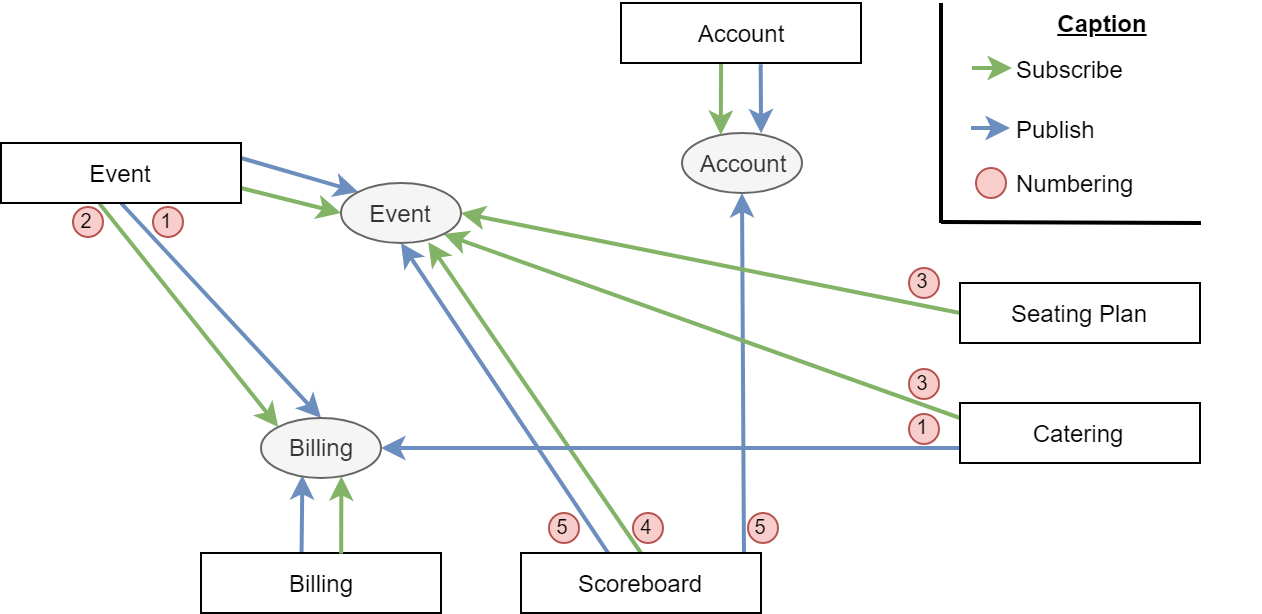
\includegraphics[width=0.9\textwidth, height=0.9\textheight, keepaspectratio]{LAN_Application_Events.png}
	\caption{LAN application asynchronous messaging events overview}
	\label{img:lanasyncevents}
\end{figure}

This concludes the architecture overview of the \ac{LAN} application.
It is important to note that this was only a high-level overview of the actual application.

\textbf{Implementation Details}

For the actual implementation, the following extensions/frameworks are used in addition to the selected technologies mentioned above:

\begin{enumerate}
	\item \textbf{express.js}: Server-side web framework for node.js (version \textit{4.17.1})
	\item \textbf{mongoose}: MongoDB object modeling framework for node.js (version \textit{5.9.17})
	\item \textbf{amqp-ts}: \ac{AMQP} communication library for node.js (version \textit{1.8.0})
	\item \textbf{bcryptjs}: Password hashing library for node.js based on \textit{bcrypt} (version \textit{2.4.3})
	\item \textbf{express-jwt}: Middleware for validating \ac{JSON} Web Tokens (version \textit{5.3.3})
	\item \textbf{Angular}: Web application framework for frontends (version \textit{9.1.9})
	\item \textbf{ng-Bootstrap}: Widgets for \textit{Angular} based on \textit{Bootstrap}, a styling framework (version \textit{6.1.0})
\end{enumerate}

In contrast to the presented services in Figure \ref{img:lansyncoverview}/\ref{img:lanasyncevents}, only three services are implemented, namely \textit{Event},\textit{ Account} and \textit{Billing}.
Although the resulting implementation would not be a viable application for an actual LAN party, it was important to demonstrate the underlying architecture for communication and event flow.
Consequently, it can be extended with additional services without many changes.

Each implemented service is bundled into an image using \textit{Docker}, which allows containerization and flexible deployment via a \textit{docker-compose} script that also handles switching environments (e.g. for development).
The current implementation consists of the following services:
\begin{enumerate}
	\item Nginx
	\item MongoDB
	\item RabbitMQ
	\item Prometheus
	\item Grafana
	\item Each implemented node.js service:
	      \subitem Account
	      \subitem Event
	      \subitem Billing
\end{enumerate}

As alluded in Figure \ref{img:lansyncoverview}, each external request is forwarded using \textit{Nginx}, including access to additional informative services (\textit{mgnt} subdomain), such as \textit{Grafana}, and direct database access (separate port) to \textit{MongoDB}.
However, the backend communicates with said services through internal endpoints, since each service is located on the same isolated network provided by \textit{Docker}.
Consequently, metric reporting and database access is restricted to the microservice environment itself.
Although metrics are already collected through Prometheus and accessible via \textit{Grafana}, a dashboard implementation was omitted in \textit{Grafana}.

Apart from the REST communication to the frontend, there is also inter-service communication over \ac{AMQP}.
The binding selected for connecting a queue to an exchange entity is a regular expression (topic exchange).
Each event has its own expression to synchronize with the services, such as \textit{account.created}, which means that the main topic is \enquote{account} and the associated sub topic is \enquote{created}.
Furthermore each service listening/consuming a queue is implemented in a way that same events can be received more than once, but only the first time is of relevance.
This implementation detail is important, as the implementation of the \ac{AMQP} protocol in this work uses a \textit{at-least-once} \ac{QoS}.

An exemplary flow of both synchronous and asynchronous messages across the whole architecture is shown in Figure \ref{img:registeraccountevent_sequence}.
The synchronous calls over REST are highlighted in blue, whereas the asynchronous publishing of messages using \ac{AMQP} are highlighted in orange.
Moreover, the data sent in each step is also shown, whereas not all internal functions of each service are represented here .
For a complete list of implemented and used events, as well as available REST endpoints, see \ref{chp:appendix:implementedRest} and \ref{chp:appendix:implementedEvent} in the appendix.

\begin{figure}
	\centering
	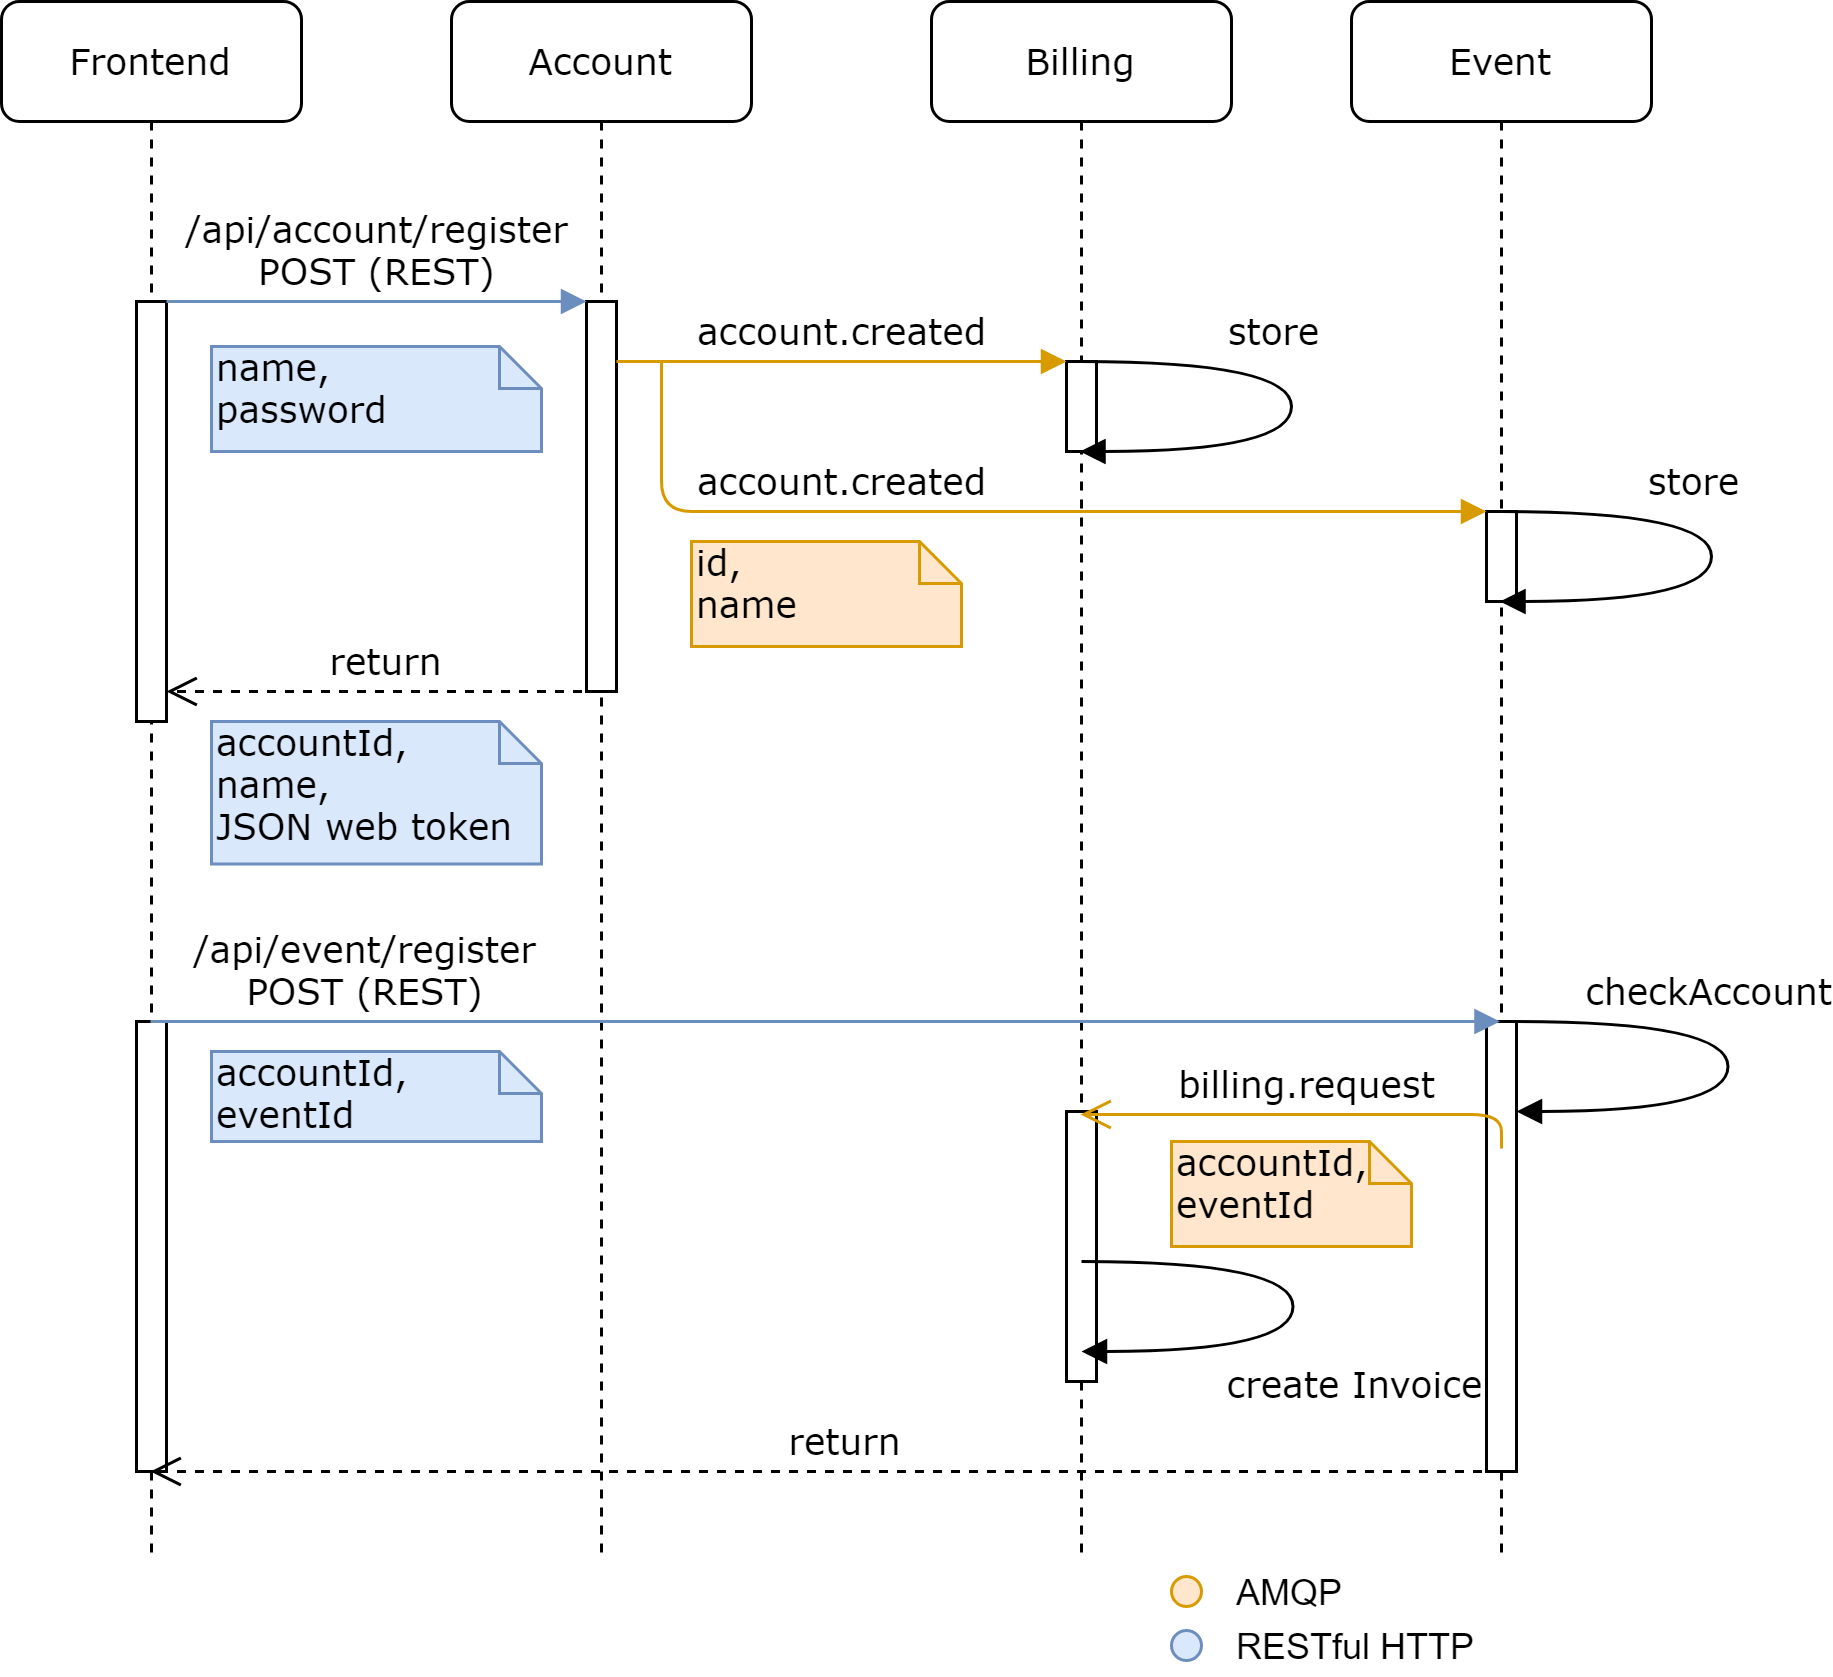
\includegraphics[width=\textwidth, height=0.6\textheight, keepaspectratio]{registeraccountevent_sequence.png}
	\caption{Example of registering account and registering for an event}
	\label{img:registeraccountevent_sequence}
\end{figure}
